\documentclass[../Bitcoin Blink.tex]{subfiles}
\graphicspath{{\subfix{../assets/images/}}}
\begin{document}
\subsection{Renting}
\begin{figure}[h]
\begin{center}
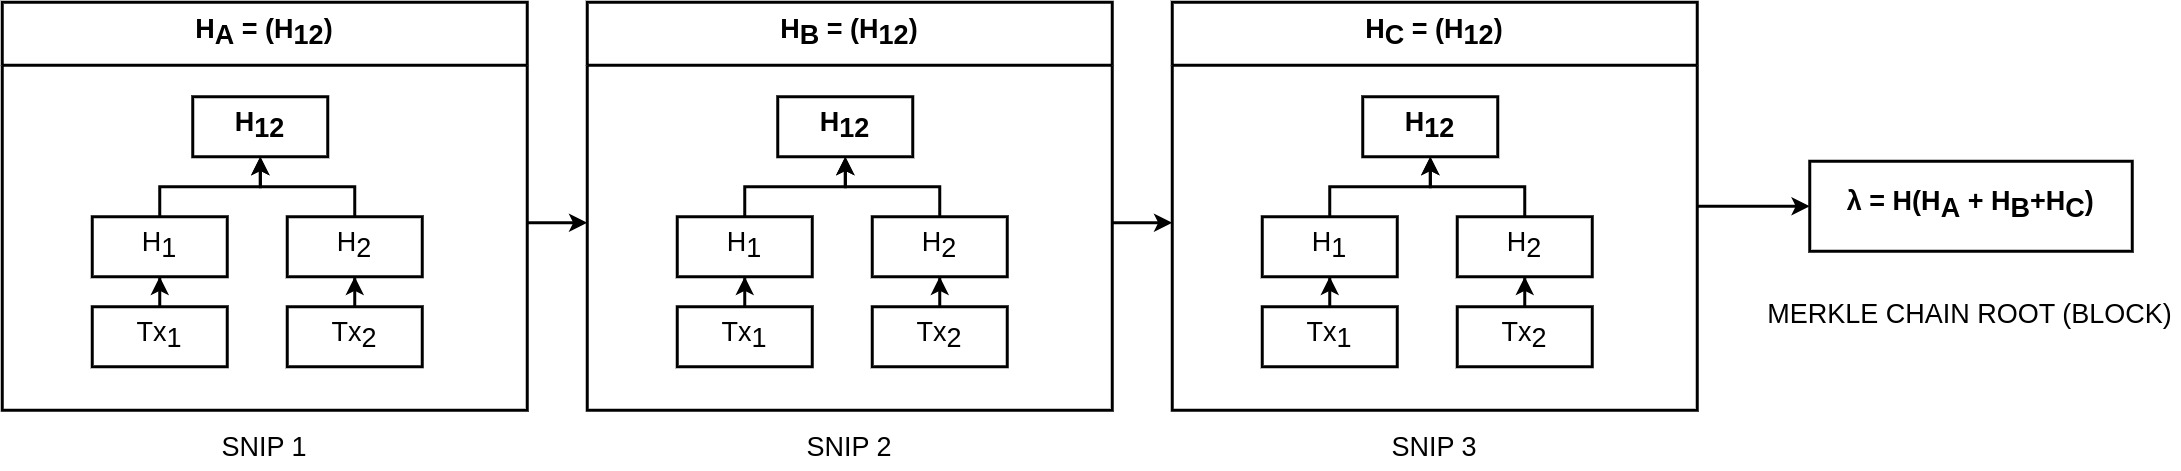
\includegraphics[width=13cm]{merklechain}
\caption{Merkle Chain}
\end{center}
\end{figure}
Instead of taking the Merkle roots of all the transactions inside a block, a snip's Merkle root is taken and linearly hashed to find the Merkle Chain root. Since snips can be rejected by validators and cannot be tampered once it is streamed to ring validators, it is unsure to predict a Merkle chain root giving it a purely randomized value. Inside a snip contains parsed transactions whose hashes are taken to find the snip's Merkle root can be pruned if the UTXOs are spent, burnt, or expired. Each UTXO expiry block height is embedded in its script, and can be scanned by nodes, and pruned to optimize their data storage. Client Wallets can store each of their users' transaction history and can be audited onchain using Merkle chain roots. Renting rates can be given in market price independently voted by producer nodes per byte per block. Users cannot directly pay for rent, but rather each new UTXO created is charged a transfer fee in the range of 0.05\% - 0.005\% decided based on the total volume of all transactions settled on previous blocks.
%Change equation from epochs to recent two blocks

 Transfer fee charges more fees for higher value utxos and less for lesser value utxos bringing ease to transact for retailers. Each UTXO's transfer fee will set an expiry date to itself. UTXOs doing state updates will not be charged where users can combine UTXOs to a single balance holding UTXO with increased expiry value. This encourages users to store a single UTXO per wallet reducing transaction fees and also incentivizes nodes, clients, etc by saving disk space.  
\end{document}
